\documentclass[journal,12pt,twocolumn]{IEEEtran}
\usepackage{setspace}
\usepackage{gensymb}
\singlespacing
\usepackage[cmex10]{amsmath}

\usepackage{amsthm}
\usepackage{hyperref}
\hypersetup{
    colorlinks=true,
    linkcolor=blue,
    filecolor=magenta,      
    urlcolor=cyan,
}

\urlstyle{same}
\usepackage{mathrsfs}
\usepackage{txfonts}
\usepackage{stfloats}
\usepackage{bm}
\usepackage{cite}
\usepackage{cases}
\usepackage{subfig}

\usepackage{longtable}
\usepackage{multirow}

\usepackage{enumitem}
\usepackage{mathtools}
\usepackage{steinmetz}
\usepackage{tikz}
\usepackage{circuitikz}
\usepackage{verbatim}
\usepackage{tfrupee}
\usepackage[breaklinks=true]{hyperref}
\usepackage{graphicx}
\usepackage{tkz-euclide}

\usetikzlibrary{calc,math}
\usepackage{listings}
    \usepackage{color}                                            %%
    \usepackage{array}                                            %%
    \usepackage{longtable}                                        %%
    \usepackage{calc}                                             %%
    \usepackage{multirow}                                         %%
    \usepackage{hhline}                                           %%
    \usepackage{ifthen}                                           %%
    \usepackage{lscape}     
\usepackage{multicol}
\usepackage{chngcntr}
\usepackage{mdframed}
\DeclareMathOperator*{\Res}{Res}

\renewcommand\thesection{\arabic{section}}
\renewcommand\thesubsection{\thesection.\arabic{subsection}}
\renewcommand\thesubsubsection{\thesubsection.\arabic{subsubsection}}

\renewcommand\thesectiondis{\arabic{section}}
\renewcommand\thesubsectiondis{\thesectiondis.\arabic{subsection}}
\renewcommand\thesubsubsectiondis{\thesubsectiondis.\arabic{subsubsection}}


\hyphenation{op-tical net-works semi-conduc-tor}
\def\inputGnumericTable{}                                 %%

\lstset{
%language=C,
frame=single, 
breaklines=true,
columns=fullflexible
}

\usepackage{chngcntr}
\counterwithin{figure}{section}

\title{AI5002}
\author{TUHIN DUTTA}
\date{January 2021}

\begin{document}
\newtheorem{theorem}{Theorem}[section]
\newtheorem{problem}{Problem}
\newtheorem{proposition}{Proposition}[section]
\newtheorem{lemma}{Lemma}[section]
\newtheorem{corollary}[theorem]{Corollary}
\newtheorem{example}{Example}[section]
\newtheorem{definition}[problem]{Definition}

\newcommand{\BEQA}{\begin{eqnarray}}
\newcommand{\EEQA}{\end{eqnarray}}
\newcommand{\define}{\stackrel{\triangle}{=}}
\bibliographystyle{IEEEtran}
\raggedbottom
\setlength{\parindent}{0pt}
\providecommand{\mbf}{\mathbf}
\providecommand{\pr}[1]{\ensuremath{\Pr\left(#1\right)}}
\providecommand{\qfunc}[1]{\ensuremath{Q\left(#1\right)}}
\providecommand{\sbrak}[1]{\ensuremath{{}\left[#1\right]}}
\providecommand{\lsbrak}[1]{\ensuremath{{}\left[#1\right.}}
\providecommand{\rsbrak}[1]{\ensuremath{{}\left.#1\right]}}
\providecommand{\brak}[1]{\ensuremath{\left(#1\right)}}
\providecommand{\lbrak}[1]{\ensuremath{\left(#1\right.}}
\providecommand{\rbrak}[1]{\ensuremath{\left.#1\right)}}
\providecommand{\cbrak}[1]{\ensuremath{\left\{#1\right\}}}
\providecommand{\lcbrak}[1]{\ensuremath{\left\{#1\right.}}
\providecommand{\rcbrak}[1]{\ensuremath{\left.#1\right\}}}
\theoremstyle{remark}
\newtheorem{rem}{Remark}
\newcommand{\sgn}{\mathop{\mathrm{sgn}}}

\providecommand{\res}[1]{\Res\displaylimits_{#1}} 

%\providecommand{\norm}[1]{\lVert#1\rVert}
\providecommand{\mtx}[1]{\mathbf{#1}}
\providecommand{\fourier}{\overset{\mathcal{F}}{ \rightleftharpoons}}
%\providecommand{\hilbert}{\overset{\mathcal{H}}{ \rightleftharpoons}}
\providecommand{\system}{\overset{\mathcal{H}}{ \longleftrightarrow}}
	%\newcommand{\solution}[2]{\textbf{Solution:}{#1}}
\newcommand{\solution}{\noindent \textbf{Solution: }}
\newcommand{\cosec}{\,\text{cosec}\,}
\providecommand{\dec}[2]{\ensuremath{\overset{#1}{\underset{#2}{\gtrless}}}}
\newcommand{\myvec}[1]{\ensuremath{\begin{pmatrix}#1\end{pmatrix}}}
\newcommand{\mydet}[1]{\ensuremath{\begin{vmatrix}#1\end{vmatrix}}}
\numberwithin{equation}{subsection}
\makeatletter
\@addtoreset{figure}{problem}
\makeatother
\let\StandardTheFigure\thefigure
\let\vec\mathbf
\renewcommand{\thefigure}{\theproblem}
\def\putbox#1#2#3{\makebox[0in][l]{\makebox[#1][l]{}\raisebox{\baselineskip}[0in][0in]{\raisebox{#2}[0in][0in]{#3}}}}
     \def\rightbox#1{\makebox[0in][r]{#1}}
     \def\centbox#1{\makebox[0in]{#1}}
     \def\topbox#1{\raisebox{-\baselineskip}[0in][0in]{#1}}
     \def\midbox#1{\raisebox{-0.5\baselineskip}[0in][0in]{#1}}
\vspace{3cm}
\title{AI5002 - Assignment 2}
\author{Tuhin Dutta\\ ai21mtech02002}
\maketitle
\newpage
\bigskip
\renewcommand{\thefigure}{\theenumi}
\renewcommand{\thetable}{\theenumi}
\begin{mdframed}
Download code and LaTeX from below hyperlinks\\
1. \href{https://github.com/Tauhait/AI5002/Assignment-2/Codes}{Code}


2. \href{https://github.com/Tauhait/AI5002/Assignment-2/LaTeX}{LaTeX}
\end{mdframed}
\subsection*{\boldsymbol{Problem\ 1.18.}}
Two players, Sangeeta and Reshma, play a tennis match. It is known that the probability of Sangeeta winning the match is 0.62. What is the probability of Reshma winning the match?
\subsection*{\boldsymbol{Solution}}\\

Given, Probability of Sangeeta winning the match\ $P$ (S_w) = 0.62.\\

Then Probability of Reshma winning the match (i.e, Probability of Sangeeta not winning the match.) be $P$ (\overline{S_w}).\\

We know,\\

$P$\ (S_w)\ +\ $P$\ (\overline{S_w})\ =\ 1\\

\implies 0.62\ +\ $P$\ (\overline{S_w})\ =\ 1\\
\begin{mdframed}
\implies $P$\ (\overline{S_w})\ =\ 0.38\\
\end{mdframed}
\subsection*{This is a Bernoulli distribution whose probability of win of Reshma and Sangeeta is shown in Fig 1.}\\

\begin{figure}[h!]
    \centering
    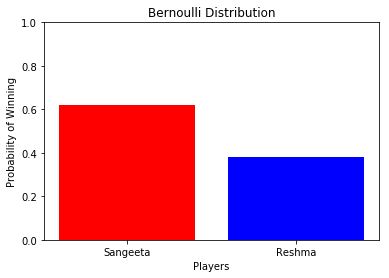
\includegraphics[width=10cm]{Assignment-2/Codes/Figures/bern_1_18.png}
    \caption*{Fig 1: Bernoulli distribution of Reshma's winning}
\end{figure}
\\
\subsection*{\boldsymbol{Problem\ 1.19.}}
Harpreet tosses two different coins simultaneously (say, one is of rupee 1 and other of rupee 2). What is the probability that she gets at least one head?
\subsection*{\boldsymbol{Solution}}\\

When two coins are tossed, then 
the set of all possible outcomes would be = \{HH, HT, TH, TT\}.\\

Thus, the total possible number of outcomes is given by\\
$$n\ (T)\ =\ 4.$$

Let E be the event of getting at least one head.\\

Then the set of favourable outcomes would be = \{HT, TH, HH\}.\\

So the number of favourable outcomes is given by\\
$$n\ (E)\ =\ 3.$$

\begin{mdframed}
The probability that Harpreet gets at least one head is $$
P\ (at\ least\ one\ head) = \frac{ n\ (E) }{ n\ (T) }
$$
$$
P\ (at\ least\ one\ head) = \frac{ 3 }{ 4 }
$$
$$
P\ (at\ least\ one\ head) = 0.75
$$\\
\end{mdframed}
\subsection*{This is again a Bernoulli distribution whose probability of at least one head and no head from two coin tosses is shown in Fig 2.}\\

\begin{figure}[h!]
    \centering
    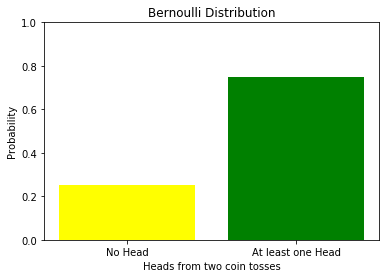
\includegraphics[width=10cm]{Assignment-2/Codes/Figures/bern_1_19.png}
    \caption*{Fig 2: Bernoulli distribution of at least one head from two coin tosses}
\end{figure}
\end{document}
